% -*- coding: utf-8 -*-

\documentclass[a4paper,dvipdfmx]{jsarticle}
\usepackage{ascmac,alltt,txfonts,url}

\usepackage[dvipdfmx]{graphicx}
\usepackage{here}

\renewcommand{\ttdefault}{cmtt}
\renewcommand{\figurename}{図} 
\renewcommand{\tablename}{表} 
\DeclareMathAlphabet{\mathtt}{OT1}{cmtt}{m}{n}
\SetMathAlphabet{\mathtt}{bold}{OT1}{cmtt}{m}{n}
\setlength{\oddsidemargin}{0cm}
\setlength{\evensidemargin}{0cm}

\makeatletter

\newdimen\@mojihaba
\settowidth{\@mojihaba}{あ}

\def\tokushu#1{%
\def\tokushutitle{#1}%
\gdef\articleHeader{\hbox to\textwidth{\rule{3\@mojihaba}{1mm}%
\hbox{\small\bf\hskip1mm \tokushutitle}\leaderfill}}
}

\newdimen \JQ	\JQ .259817mm	%%%	\JQ/\Q = 10pt/9.62216pt
\newdimen \Q	\Q  .25mm	%%%	Quarter of 1mm

\def\JarticleHeader{\rule{\textwidth}{1mm}}%
\def\JarticleTitle{{\huge\bf\@title}}
\def\JarticleAuthor{\large\begin{tabular}[t]{@{}l}\@author\end{tabular}}
\newbox\@temptitlebox

\def\verse{\let\\=\@centercr 
 \list{}{\itemsep\z@ \itemindent -1.5em\listparindent \itemindent 
 \rightmargin\leftmargin\advance\leftmargin 1.5em}\item[]}
\let\endverse\endlist
\def\quotation{\list{}{\listparindent 1.5em
 \itemindent\listparindent
 \rightmargin\leftmargin \parsep 0pt plus 1pt}\item[]}
\let\endquotation=\endlist
\def\quote{\list{}{\rightmargin\leftmargin}\item[]}
\let\endquote=\endlist
\def\abstquotation{\list{}{\listparindent 1.5em
 \itemindent\listparindent
 \leftmargin 5mm
 \rightmargin\leftmargin \parsep 0pt plus 1pt}\item[]}
\let\endabstquotation=\endlist
\def\quote{\list{}{\rightmargin\leftmargin}\item[]}
\let\endquote=\endlist

\global\def\@maketitle{\newpage \null
\hbox{\vbox to193.5\Q{\baselineskip=10mm % 193.5\Q = 9*\baselineskip
\begin{flushleft}
\JarticleHeader
% following extra vskip together with baselineskip(10mm) will produce
% appropriate 10mm/6mm gap between the rule and title
% This assumes that title is typeset with 28Q(7mm) font, and baseline
% is set 1mm above the bottom of the font.
\setbox\@temptitlebox\hbox{JarticleTitle}\ifdim\wd\@temptitlebox>\textwidth\vskip2mm\else\vskip6mm\fi
\leftskip=5mm
\JarticleTitle
\vskip6mm % to leave 10mm gap between title and author
\JarticleAuthor
\end{flushleft}\vfil}}
%\JEabstInsert
  \begin{small}
    \begin{abstquotation}
      \Jabstcontent
    \end{abstquotation}
  \end{small}
}

\long\def\Jabstract#1{\global\long\def\Jabstcontent{\noindent\ignorespaces #1}}
\def\Jabstcontent{\relax}

\makeatother

\usepackage{fancyhdr}
\pagestyle{fancy}
\lhead{Vivado Design Suiteのインストール}
\rhead{}
\rhead{\thepage{}}
\cfoot{}
\renewcommand{\headrulewidth}{0.5pt}
\pagestyle{fancy}

\Jabstract{%
\\
Vivadoをインストールして,いつでもFPGAの開発ができる環境を整えておこう.実際にFPGAを使うだけではなく,文法の確認やシミュレーションによる動作の確認にも利用できますよ.
}

\begin{document}

\title{Vivado Design Suiteのインストール}
\author{}
\date{2019年 1月14日~~第3.0版}
\maketitle

 \section{はじめに}

 ZYBO Z7-20をはじめ,XilinxのFPGAを利用するためにはXilinxの提供する開発環境Vivado Design Suite(以下Vivado)をパソコンにインストールしておく必要があります.VivadoはWindowsおよびLinuxで利用することができます.ここでは,Windows10へのインストールをステップ毎に紹介します.

 実際にFPGAを使わない場合でも,文法のチェックや合成・配置配線によるリソース使用量のチェック,シミュレーションによる動作の確認を行なうことができますのでインストールしておくと便利です.C/C++を使ったFPGA開発用のツールであるVivado HLSも一緒にインストールできます.

 \section{インストーラのダウンロード}
 まずはインストーラを,XilinxのWebページからダウンロードします.

 \begin{figure}[H]
  \begin{center}
   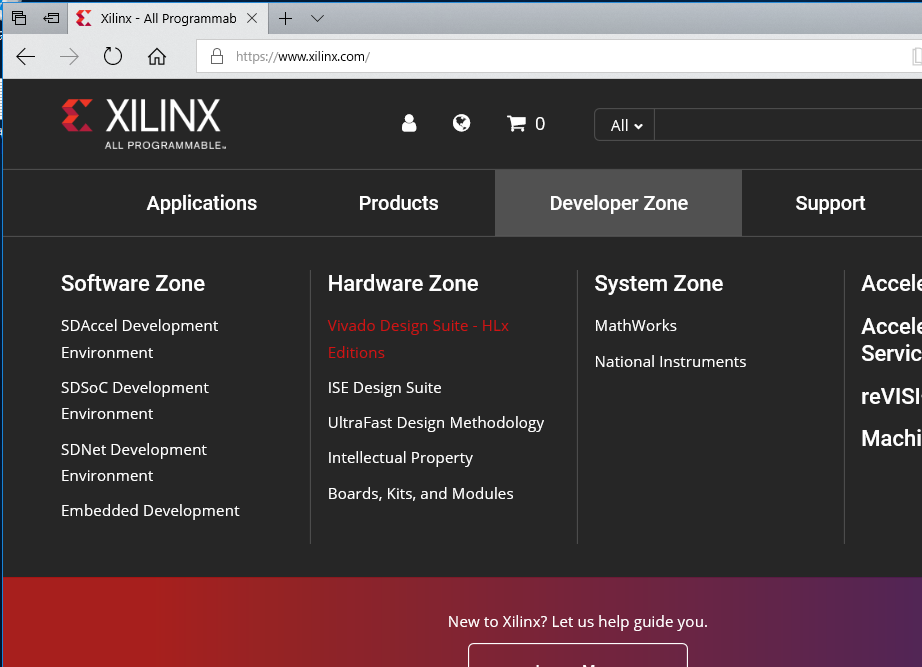
\includegraphics[width=.9\textwidth]{appendix_figures/01_xilinx_web_page.png}
  \end{center}
  \caption{XilinxのWebページを訪れ,``Developer Zone''から ``Vivado Design Suite - HLx Editions''を選ぶ}
 \end{figure}

 \begin{figure}[H]
  \begin{center}
   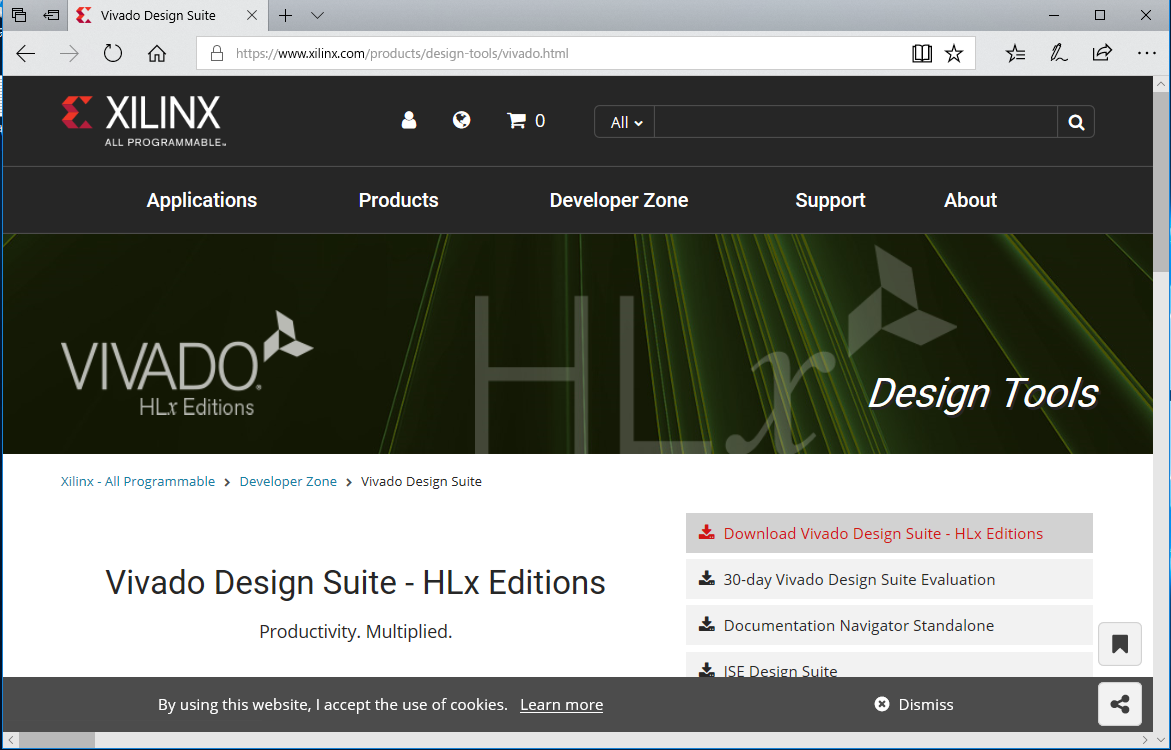
\includegraphics[width=.9\textwidth]{appendix_figures/02_xilinx_web_page.png}
  \end{center}
  \caption{``Download Vivado Design Suite - HLx Editions''を選択}
 \end{figure}

 \begin{figure}[H]
  \begin{center}
   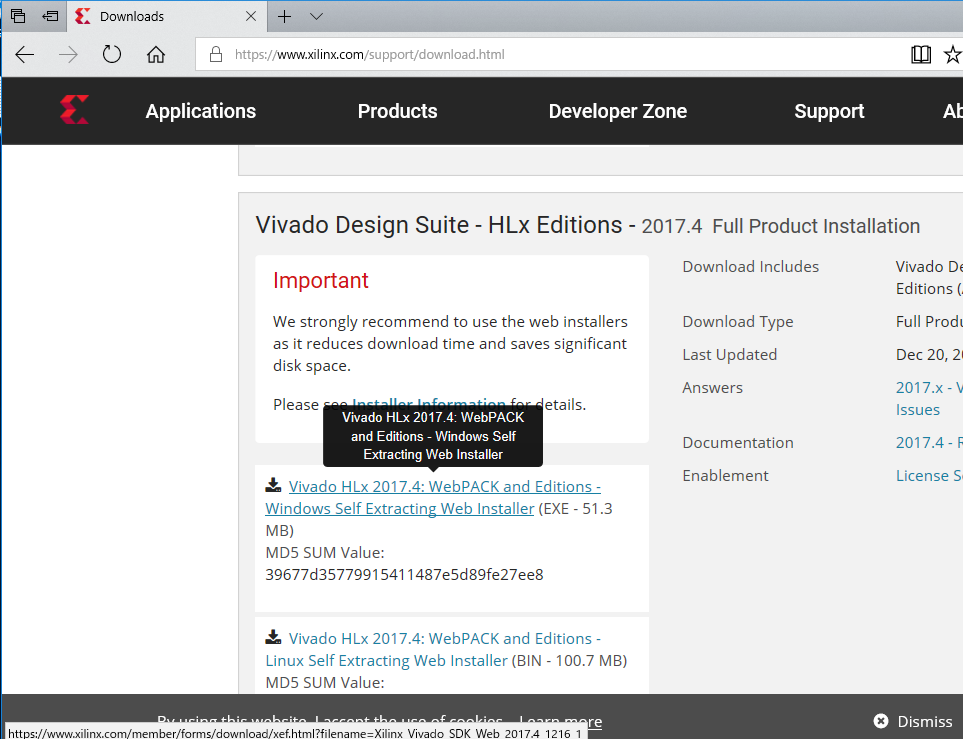
\includegraphics[width=.8\textwidth]{appendix_figures/03_xilinx_web_page.png}
  \end{center}
  \caption{ページ半程にあるWebインストーラをダウンロード.Windows用とLinux用があるので注意}
 \end{figure}

 \begin{figure}[H]
  \begin{center}
   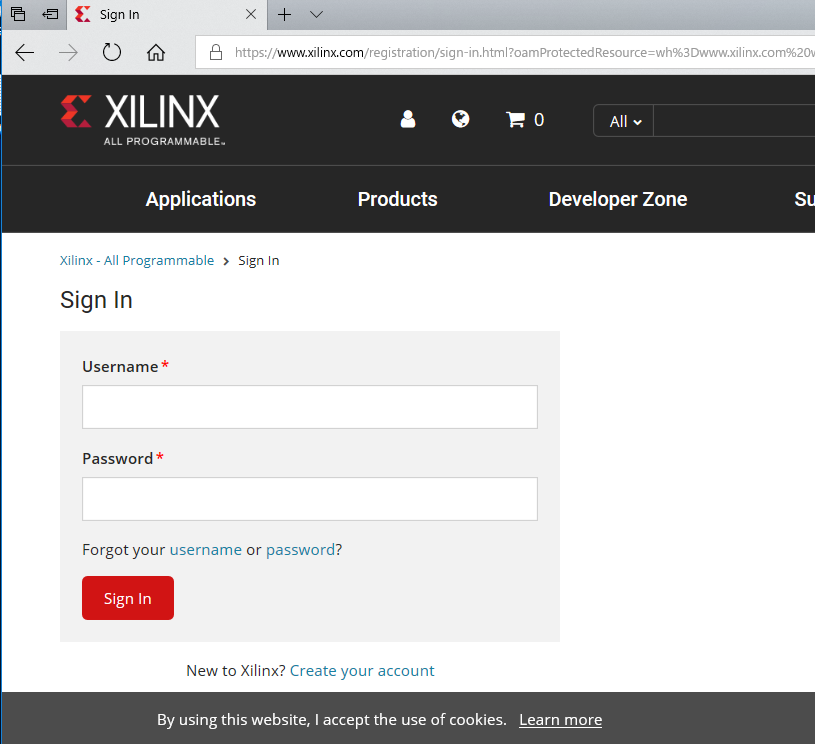
\includegraphics[width=.7\textwidth]{appendix_figures/04_xilinx_web_page.png}
  \end{center}
  \caption{ダウンロードにはユーザ登録が必要.Create your accountからアカウントを作成しましょう}
 \end{figure}

 \begin{figure}[H]
  \begin{center}
   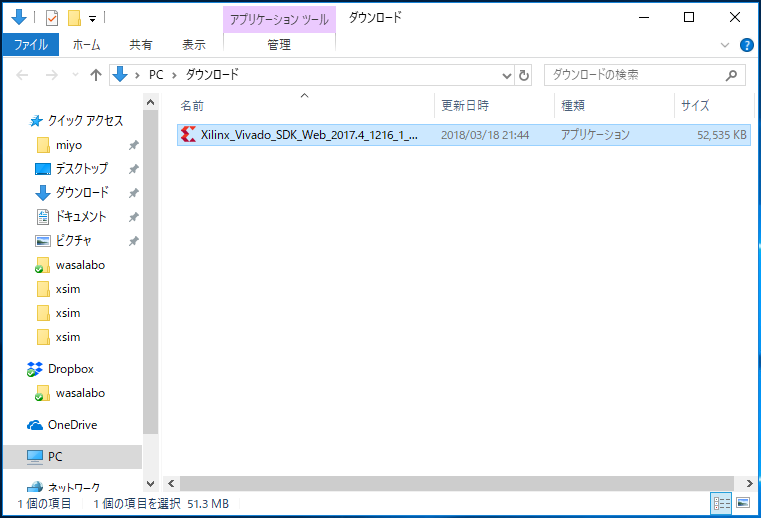
\includegraphics[width=.65\textwidth]{appendix_figures/05_installer_downloaded.png}
  \end{center}
  \caption{必要な項目を入力するとインストーラのダウンロードができます}
 \end{figure}

 \section{インストーラの実行}
 ダウンロードしたインストーラをダブルクリックで起動して,インストールしましょう.

 \begin{figure}[H]
  \begin{center}
   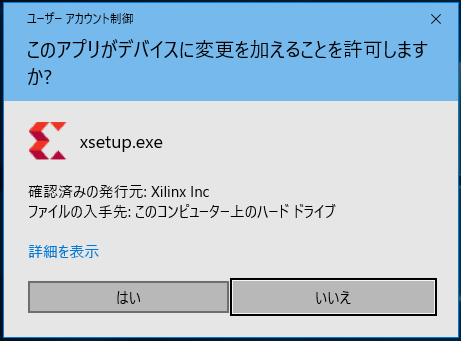
\includegraphics[width=.5\textwidth]{appendix_figures/06_installer_uac.png}
  \end{center}
  \caption{デバイスへの変更は,もちろん許可してください}
 \end{figure}

 \begin{figure}[H]
  \begin{center}
   
\includegraphics[width=.5\textwidth]{appendix_figures/07_installer_splash.png}
  \end{center}
  \caption{インストーラが起動するとスプラッシュが表示されます}
 \end{figure}

 \begin{figure}[H]
  \begin{center}
   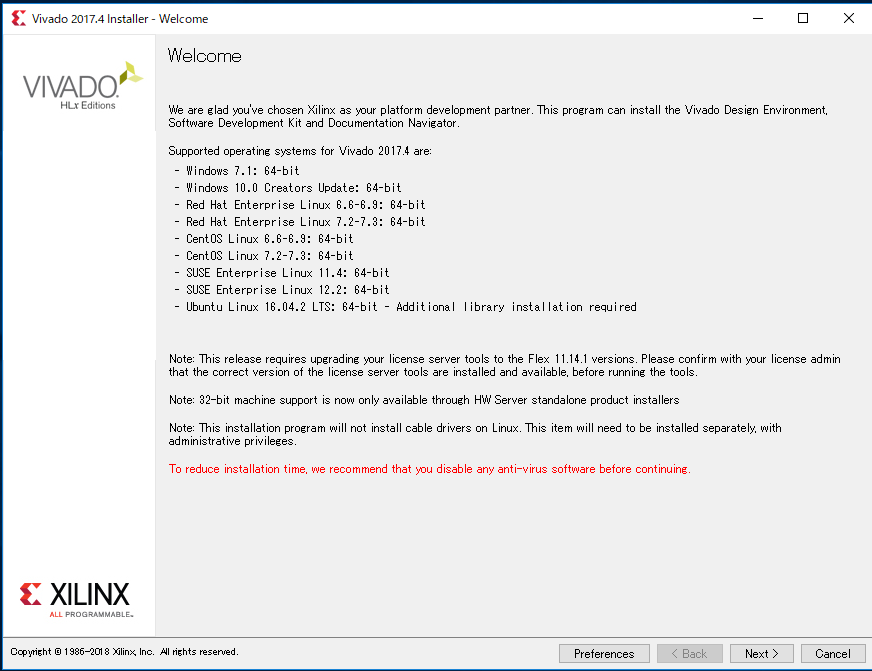
\includegraphics[width=.8\textwidth]{appendix_figures/08_installer_main.png}
  \end{center}
  \caption{インストーラが起動しました.ダイアログ下のNext$\gt$をクリックして次にすすみましょう}
 \end{figure}

 \begin{figure}[H]
  \begin{center}
   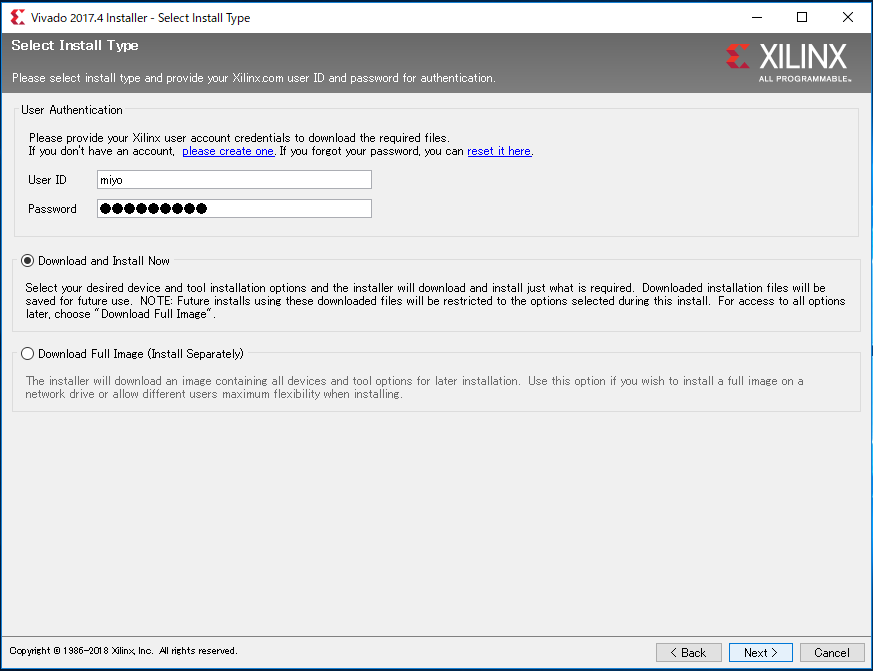
\includegraphics[width=.8\textwidth]{appendix_figures/09_installer_main.png}
  \end{center}
  \caption{インストーラのダウンロード時に入力したユーザ名とパスワードを,User IDとPasswordのテキストボックスに入力しましょう.``Download and Install Now''にチェックがはいっていることを確認して,Next$\gt$をクリックします}
 \end{figure}

 \begin{figure}[H]
  \begin{center}
   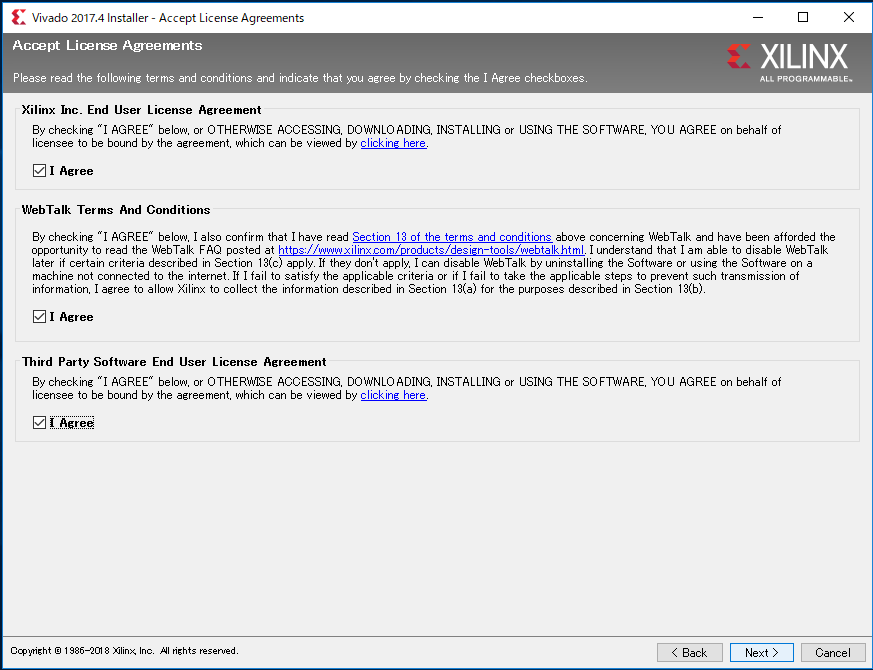
\includegraphics[width=.8\textwidth]{appendix_figures/10_installer_main.png}
  \end{center}
  \caption{インストールされる各種ソフトウェアのライセンス確認です.3箇所の``I Agree''にチェックをいれて,Next$\gt$をクリックします}
 \end{figure}

 \begin{figure}[H]
  \begin{center}
   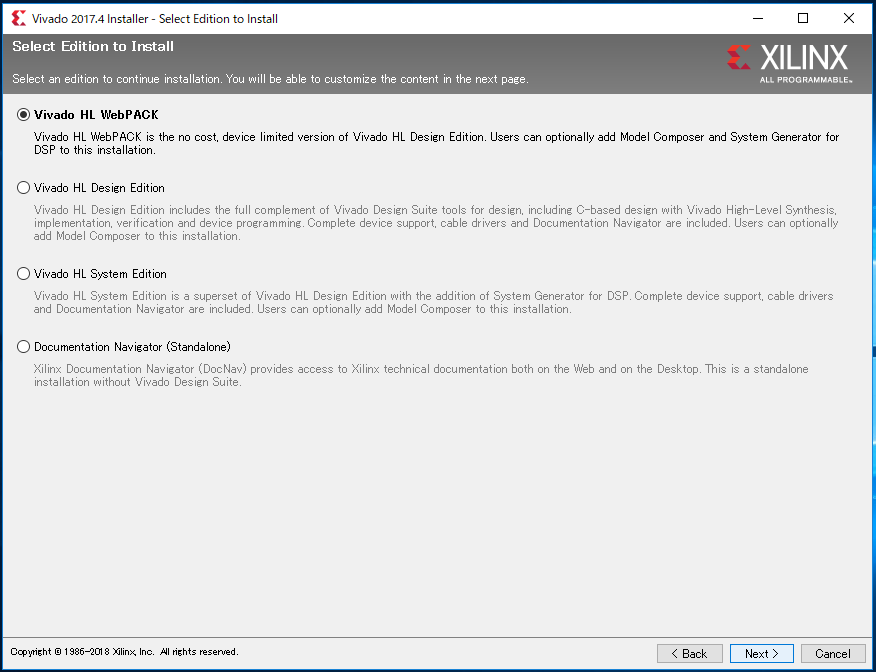
\includegraphics[width=.8\textwidth]{appendix_figures/11_installer_main.png}
  \end{center}
  \caption{同じインストーラで様々なグレードのVivadoをインストールできます.ここでは無償で利用可能な ``Vivado HL WebPACK''を選択して,Next$\gt$をクリックします.もし将来的にWebPACKが対応していない大きなFPGAを使用する可能性がある場合にはDesign Editionを選択しても構いませんが,インストール後に追加することもできます.}
 \end{figure}

 \begin{figure}[H]
  \begin{center}
   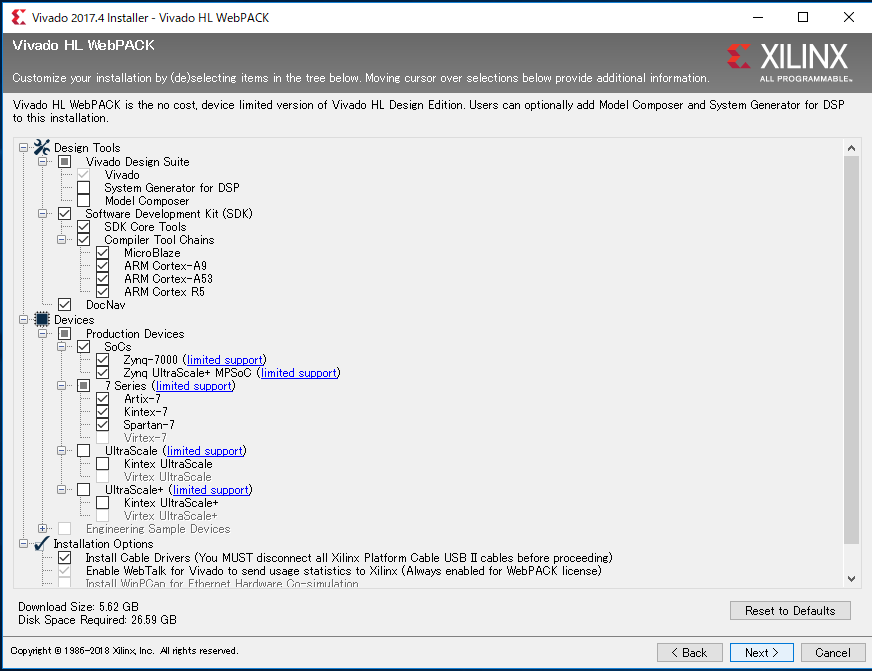
\includegraphics[width=.8\textwidth]{appendix_figures/12_installer_main.png}
  \end{center}
  \caption{インストールするツールと対象デバイスを選択します.後々のことを考えると``Software Development Kitのすべてのチェックボックスにチェックを入れておくとよいでしょう.また使用するデバイスは,少なくとも``Zynq-7000''は選択しておきます.他は選択してしなくても構いません.``Install Cable Drivers''にチェックが入っていることを確認して,Next$\gt$をクリックします.}
 \end{figure}

 \begin{figure}[H]
  \begin{center}
   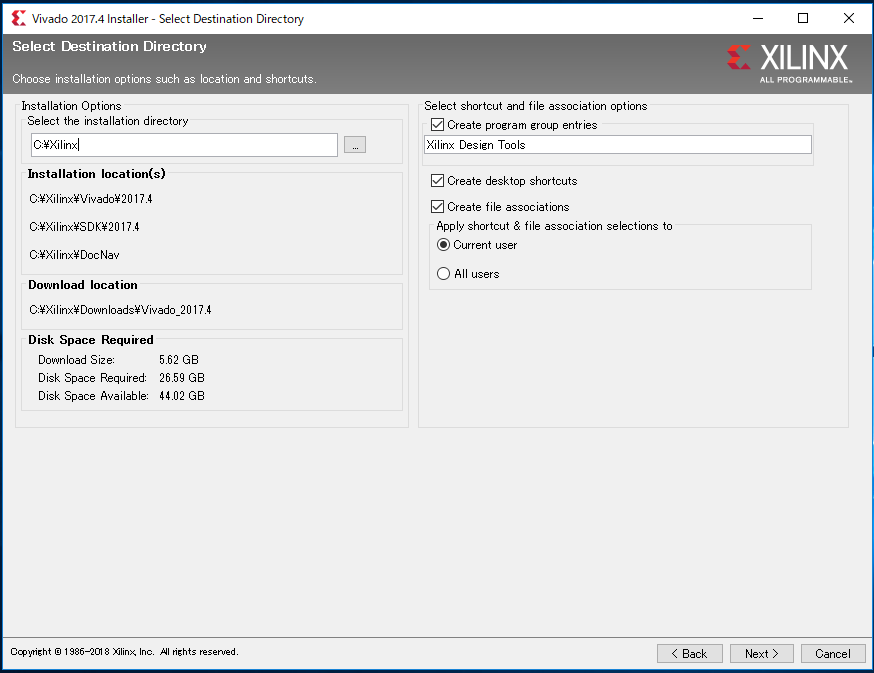
\includegraphics[width=.8\textwidth]{appendix_figures/13_installer_main.png}
  \end{center}
  \caption{インストール先の指定です.特に変更する必要はないでしょう.ここでは,今回26.59GBのディスク容量が必要になることがわかります.Next$\gt$をクリックして次にすすみます.}
 \end{figure}

 \begin{figure}[H]
  \begin{center}
   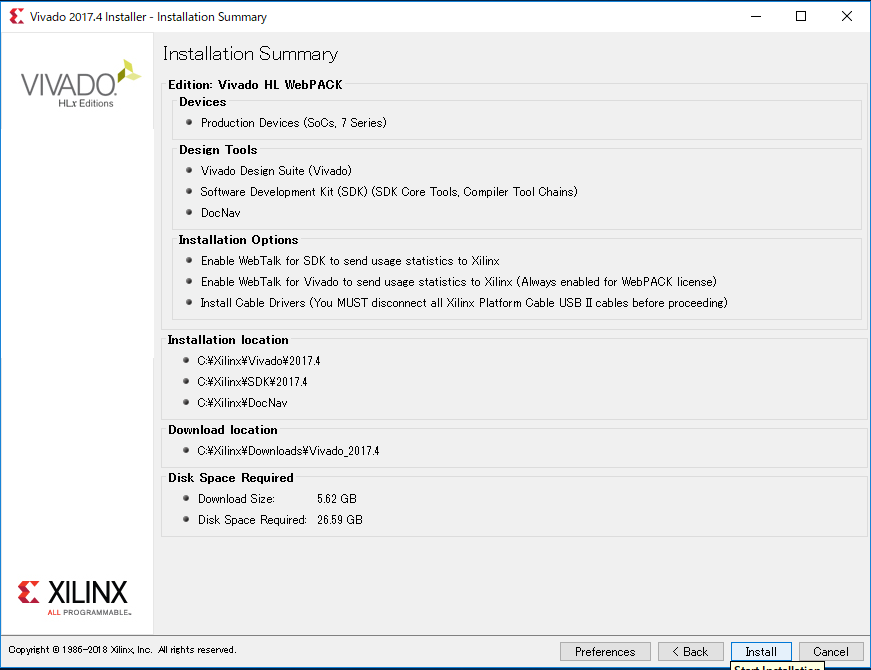
\includegraphics[width=.8\textwidth]{appendix_figures/14_installer_main.png}
  \end{center}
  \caption{インストール前の最後の確認です.Next$\gt$をクリックして次にすすみましょう.}
 \end{figure}

 \begin{figure}[H]
  \begin{center}
   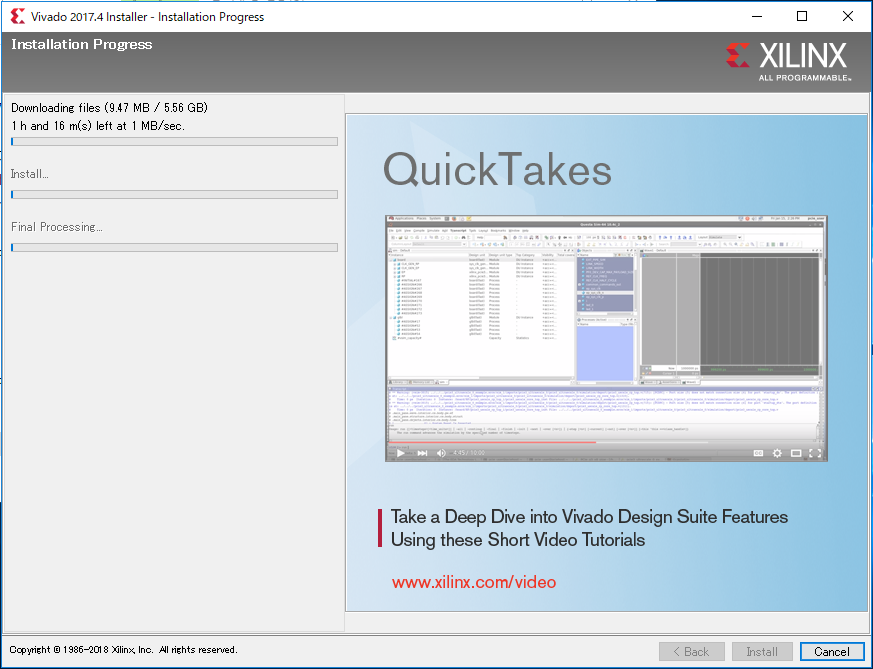
\includegraphics[width=.8\textwidth]{appendix_figures/15_installer_main.png}
   \caption{インストール進行中です.ネットワーク環境やパソコンの性能によりますが,少なくとも1-2時間程度の時間は覚悟するとよいでしょう.}
  \end{center}
 \end{figure}

 \begin{figure}[H]
  \begin{center}
   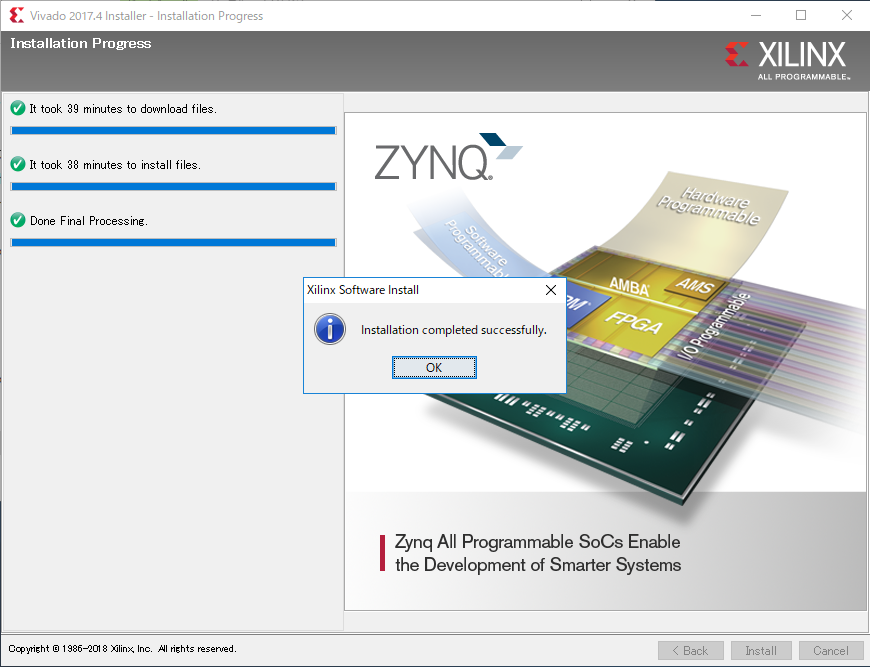
\includegraphics[width=.8\textwidth]{appendix_figures/16_installer_main.png}
   \caption{インストールが完了.この環境では1時間20分程度必要でした.}
  \end{center}
 \end{figure}

 \begin{figure}[H]
  \begin{center}
   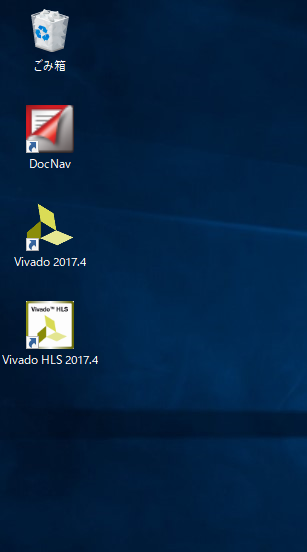
\includegraphics[width=.3\textwidth]{appendix_figures/17_installed_vivado.png}
   \caption{起動用のショートカット ``Vivado 2017.4''がデスクトップに作成されました.}
  \end{center}
 \end{figure}

 \begin{figure}[H]
  \begin{center}
   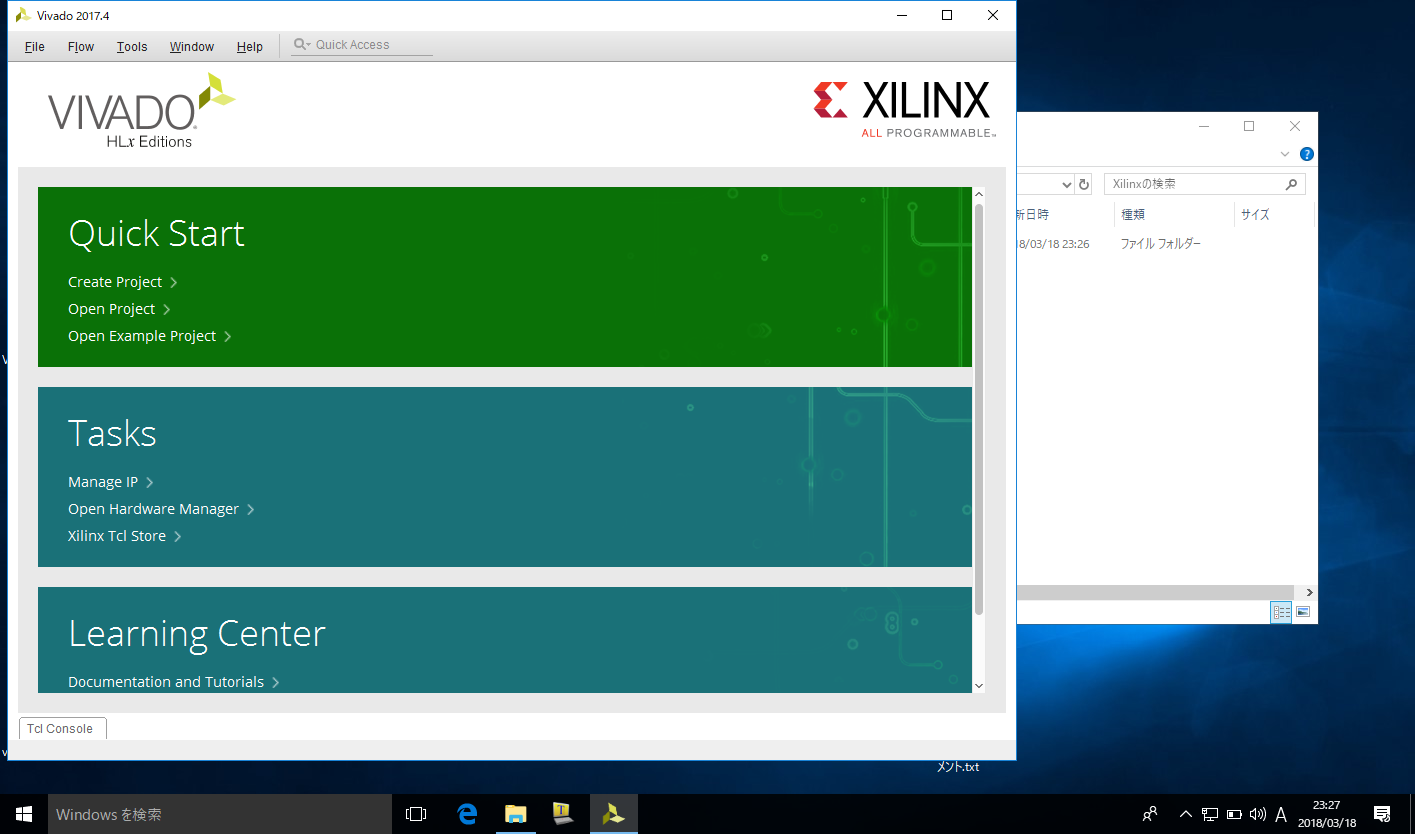
\includegraphics[width=.3\textwidth]{appendix_figures/18_installed_vivado.png}
   \caption{ショートカット ``Vivado 2017.4'' をクリックするとVivadoが起動します.}
  \end{center}
 \end{figure}

\section{ボード定義ファイルのダウンロードとインストール}
Vivadoのインストールが完了したら,最後にDigilentの提供するボード定義ファイルをダウンロードしてインストールしましょう.これをインストールしておくと,Digilentの提供するFPGAボードに搭載されているFPGAやメモリ,I/Oの構成などのボード情報をライブラリから呼び出すことができるようになり,開発が簡単になります.

まず,DigilentのWebページである,Installing Vivado and Digilent Board Files(\url{https://reference.digilentinc.com/vivado/installing-vivado/start})の半ほどにある,archiveというリンク(https://github.com/Digilent/vivado-boards/archive/master.zip)からダウンロードします.

ダウンロードしたら,すべて展開し,展開してできた,vivado-boards-master\yen vivado-boards-master\yen newの下にあるboard\_filesをコピーし,C:\yen Xilinx\yen Vivado\yen 2017.4\yen data\yen boardsにはりつけましょう.最初からboard\_filesフォルダは存在していますが,構わずはりつけると,Digilentの提供するボード定義ファイルが追加されます.

 \begin{figure}[H]
  \begin{center}
   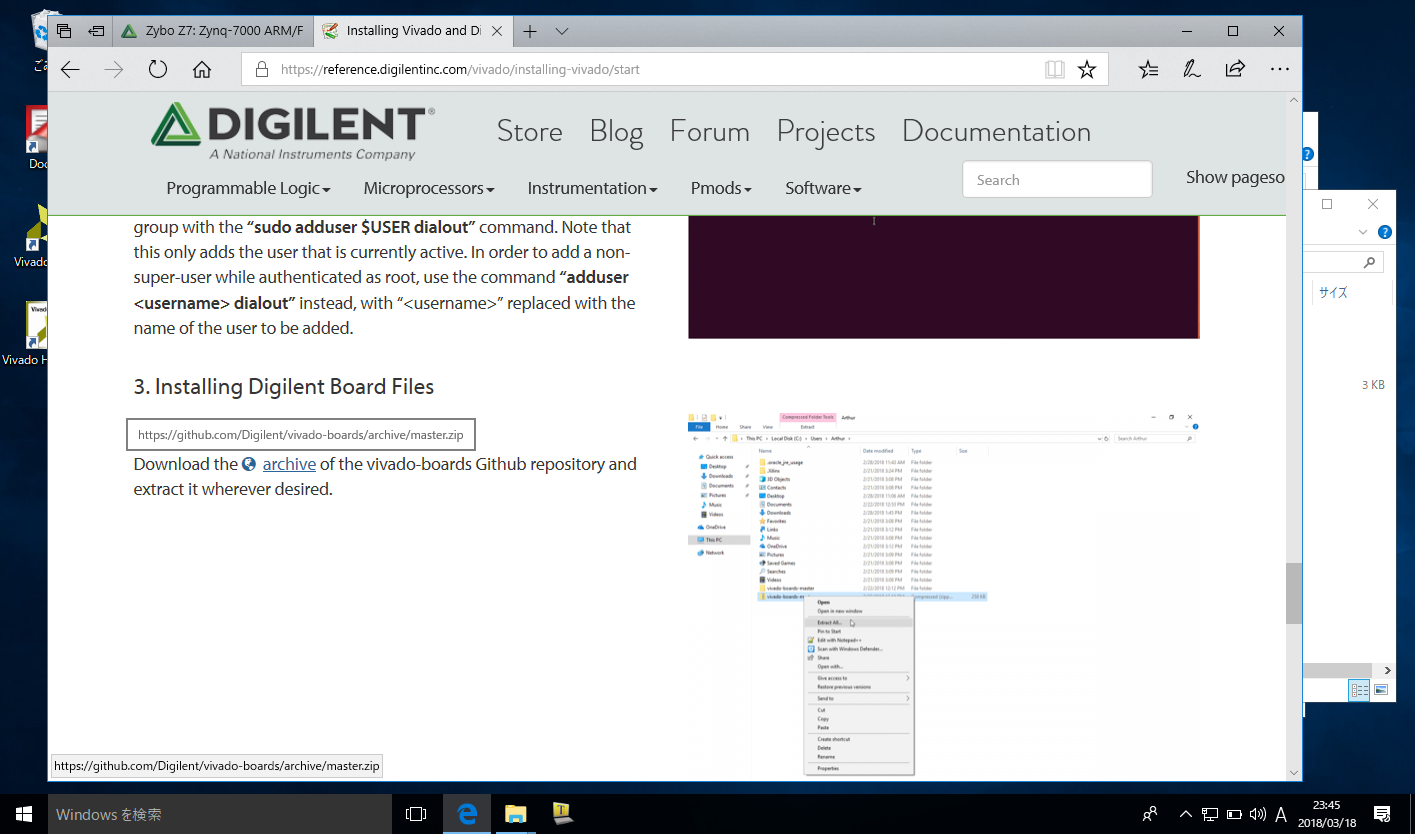
\includegraphics[width=.8\textwidth]{appendix_figures/19_download_archive.png}
  \end{center}
   \caption{まずは,アーカイブファイルをダウンロードする.}
 \end{figure}
 \begin{figure}[H]
  \begin{center}
   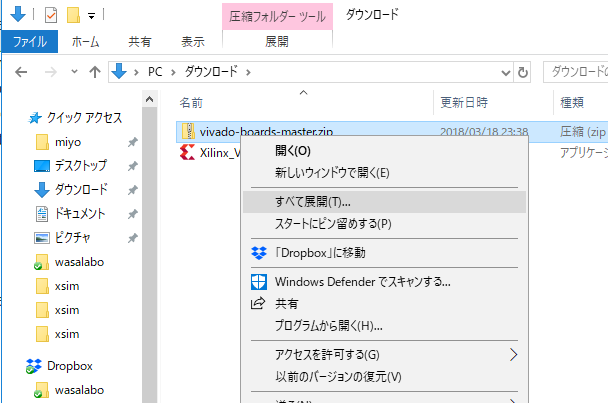
\includegraphics[width=.6\textwidth]{appendix_figures/20_extract_archive.png}
  \end{center}
   \caption{ダウンロードしたファイルを展開する}
 \end{figure}
 \begin{figure}[H]
  \begin{center}
   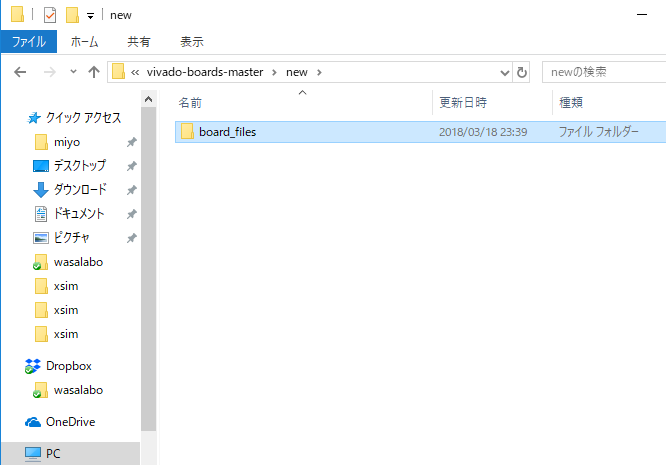
\includegraphics[width=.6\textwidth]{appendix_figures/21_board_file.png}
  \end{center}
  \caption{展開後の vivado-boards-master\yen vivado-boards-master\yen new の board\_file をコピー}
 \end{figure}
 \begin{figure}[H]
  \begin{center}
   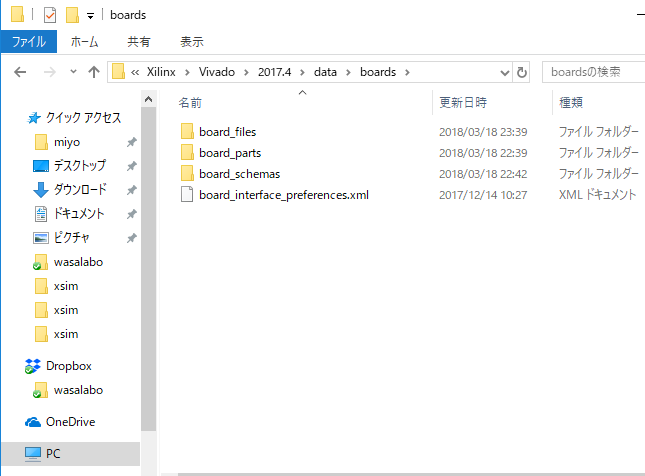
\includegraphics[width=.6\textwidth]{appendix_figures/22_dest_folder.png}
  \end{center}
  \caption{ C:\yen Xilinx\yen Vivado\yen 2017.4\yen data\yen boards にはりつける}
 \end{figure}


\end{document}
